%!TEX root = ../../main.tex

\chapter{Entwurf} % oder Entwicklung
In diesem Kapitel wird der Entwurf und die Architektur des Programms beschrieben. Zuerst wird beschrieben, welche Anforderungen es an das Programm gibt. Danach werden die verwendeten Architekturpatterns erläutert. Darauf folgt ein Kapitel zur Architektur des Backends in dem beschrieben wird, wie die Endpunkte der API gestaltet sind, welche Technologien verwendet werden und wie der innere Aufbau der API aussieht. Anschließend werden die wichtigsten Prozesseabläufe dargestellt und schließlich, wie das Projekt auf einem Server aufgesetzt wird.

\section{Anforderungen}
Das Programm soll eine Webanwendung sein auf der Nutzer mit einer benutzerfreundlichen Oberfläche verschiedene Eröffnungen betrachten und trainieren können. Es soll dabei als zentraler Ort dienen um Eröffnungen nachzuschauen und sein Gedächtnis aufzufrischen. Die Anwendung unterstützt Lernende, indem sie personalisiert Vorschläge gibt, welche Eröffnungen erneut geübt werden sollen. Folgende Features sollen implementiert werden:

\begin{itemize}
    \item Login: Ein Nutzer kann sich bei der Anwendung anmelden.
    \item Registrieren: Ein Nutzer kann einen Account anlegen.
    \item Spielumfang: Die Anwendung bietet zu Beginn jeweils mindestens eine Eröffnung für die weißen und für die schwarzen Figuren an.
    \item Lernmodus: Ein Nutzer kann eine Eröffnung auswählen und anschließend verschiedene Zugfolgen und Varianten der Eröffnung betrachten.
    \item Übungsmodus: Ein Nutzer kann eine Eröffnung auswählen und muss dann die Figuren einer Farbe nach der Zugfolge der Eröffnung bewegen. Der Computer spielt dabei die Züge des Gegners.
    \item Übungsmodus Hinweise: Während dem Üben hat ein Nutzer die Möglichkeit sich Hinweise geben zu lassen.
    \item Übungsmodus Erweiterung: Ein Nutzer hat die Möglichkeit nach einer Eröffnung mit oder ohne Dekomposition das Spiel zu Ende zu spielen gegen einen Computergegner.
    \item Vorschläge: Ein Nutzer bekommt Vorschläge welche Eröffnung trainiert werden soll.
    \item Statistik: Ein Nutzer kann sich Statistiken zu den Eröffnungen anschauen. Dazu zählt die Anzahl an richtigen und falschen Übungsdurchläufen. Diese Statistik wird auch zur Erstellung der Vorschläge verwendet.
\end{itemize}

\section{Patterns}
In diesem Kapitel werden architekturübergreifende Patterns vorgestellt, die unabhängig vom gewählten Architekturstil eingesetzt werden können. Sie tragen dazu bei, den Code besser strukturiert, wartbar und erweiterbar zu gestalten. Dazu gehören das Repository Pattern und Dependency Injection. Beide Patterns werden im Folgenden erläutert.

\subsection{Dependency Injection}
Das Ziel von Dependency Injection ist es, Softwarekomponenten lose zu verbinden. Klassen sollen, anstatt selbst Objekte zu erstellen, beschreiben, welche Funktionalität sie benötigen. Diese Beschreibung findet über Interfaces (Schnittstellen) statt. Diese definieren, welche Funktionen benötigt werden. In der einfachsten Form, der puren Dependency Injection, werden die Objekte über den Konstruktor übergeben. Häufig wird allerdings ein Dependency Injection Container verwendet um die benötigten Objekte in eine Klasse zu \enquote{injizieren}.

Das Verwenden von Dependency Injection bietet einige Vorteile. Zum einen ermöglicht es Late Binding, also das späte definieren von Verbindungen. So kann zum Beispiel über eine Konfigurationsdatei im Nachhinein geändert werden, welche Klasse für die Instanzierung einer bestimmten Abhängigkeit verwendet wird. Zum anderen erleichtert es auch die Erweiterung eines Programms. Zusätzliche Features können implementiert werden, indem einzelne Abhängigkeiten angepasst oder ersetzt werden, ohne dass sich das Interface verändert. Auch für Tests ist es dadurch einfach, die tatsächlichen Abhängigkeiten durch Testdoubles zu ersetzen und Klassen isoliert zu testen. Das ist vor allem bei Unittests nützlich. Durch die Definierung von klaren Schnittstellen, ist auch die parallele Entwicklung an unterschiedlichen Modulen möglich. Wenn man sich zusätzlich an die Regel hält, dass jede Klasse nur einen Zweck hat, verbessert Dependency Injection auch die Wartbarkeit. Es ist dann oft möglich neue Features umzusetzen, indem vorhandene Klassen durch Einbindung neuer Klassen erweitert werden.
\cite{seemann_dependency_2019}

\subsection{Repository Pattern}
Um die Datenspeicherung von dem Rest des Backends zu trennen wird das Repository Pattern angewendet. Bei diesem Pattern wird eine Repository-Klasse erstellt, welche die Abfragelogik enthält. Nach außen werden nur abstrakte domänenspezifische Funktionen exponiert, wie zum Beispiel \lstinline{GetUser(id: int): User} oder \lstinline{CreateUser(name: string, password: string)}. Die Implementierung dieser Klasse sorgt dafür, dass die entsprechenden Daten gefunden, aktualisiert oder hinzugefügt werden. Diese Abfragen können zum Beispiel komplexe SQL-Abfragen sein oder auch das Lesen einer Datei. In diesem Projekt wird jede Repository durch ein Interface definiert. Das ermöglicht es die jeweiligen Implementierungen mittels Dependency Injection zu ersetzen. \cite{evans_domain-driven_2004}

\section{Architektur}
Die Architektur ist in mehrere verschiedene Bestandteile aufgeteilt. Die zentrale Aufteilung besteht zwischen Backend und Frontend. In dieser Arbeit wird nur das Backend betrachtet. In \autoref{fig:components} ist ein Überblick über die Architektur zu sehen. Das Frontend greift auf eine \ac{REST}-API zu.
Die API ist wiederum aufgeteilt in die vier Bestandteile Eröffnungen, Nutzerdaten, Statistiken und die Schachengine.
Die Bestandteile werden in den folgenden Unterkapiteln näher erklärt.
% Der Bestandteil Eröffnungen ist für alles zuständig, wofür die Daten für Eröffnungen benötigt werden. Dazu gehört also das Lernen und Üben von Eröffnungen. Der Bestandteil Nutzerdaten ist notwendig um das Registrieren und den Login zu ermöglichen und die Statistiken sind nützlich um den Fortschritt der Spieler zu verfolgen und ermöglichen eine personalisierte Anpassung der Lernerfahrung. Die Schachengine ist notwendig für das Spielen gegen den Computer.

\begin{figure}[h]
    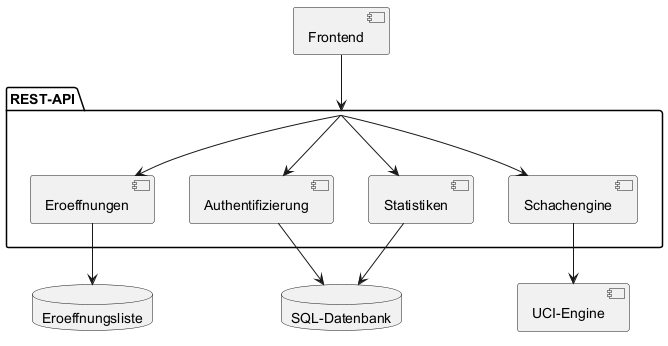
\includegraphics[width=\linewidth]{images/diagrams/components.png}
    \caption{Komponentendiagramm}
    \label{fig:components}
\end{figure}

\subsection{REST-API}
Die API wird in C\# realisiert. Mit dem ASP.NET Core Framework wird eine controllerbasierte Web-API erstellt. Das bedeutet, dass die Controller und die Daten voneinander getrennt werden. Die Architektur ist ähnlich, wie eine Model View Controller Architektur, mit dem Unterschied, dass es keine View gibt. Die View wird separat im Frontend entwickelt. Die Controller und die Models sind im Backend vorhanden. Die Controller offenbaren die API-Endpunkte nach außen und die Models modellieren die Daten. Für die vier unterschiedlichen Bereiche des Backends existiert jeweils ein dazugehöriger Controller. Jeder Controller repräsentiert dabei einen Wurzelendpunkt in der REST-API. Damit gibt es die vier Wurzelendpunkte \lstinline{/engine}, \lstinline{/openings}, \lstinline{/users} und \lstinline{/stats}. Ein Controller-Endpunkt gibt immer ein \lstinline{IActionResult} zurück. Wenn in der Implementierung ein anderer Datentyp zurückgegeben wird, kümmert sich das Framework darum, dass er umgewandelt wird. Das resultiert in einem \lstinline{OkObjektResult} mit dem Statuscode 200 und dem zurückgegebenen Objekt als Wert. Dieses Objekt wird vor der Antwort in JSON umgewandelt. Um Verständlichkeit der nachfolgenden Klassendiagramme zu erhöhen wird nur der Datentyp dieses Objekts dargestellt. In manchen Fällen ist es auch möglich, dass statt des Datentyps eine Antwort mit Fehlercode und anderen Daten übergeben wird. Das wird an den entsprechenden Stellen beschrieben und ist auch in der OpenAPI Dokumentation zu sehen.
% TODO im Code umsetzen

\subsection{Eröffnungen}
\label{cp:openings}
Der Bestandteil Eröffnungen ist für alles zuständig, wofür die Daten der Eröffnungen benötigt werden. Dazu gehört also das Lernen und Üben von Eröffnungen. \autoref{fig:cd_opening} zeigt die dazugehörigen Klassen.

\subsubsection{OpeningController}
Der OpeningController definiert alle Endpunkte unter der URI \lstinline{/openings}.
Jede public Funktion der Klasse ist in diesem Fall für einen Endpunkt zuständig. Die Zuteilung ist folgendermaßen gestaltet:

\begin{figure}[htb]
  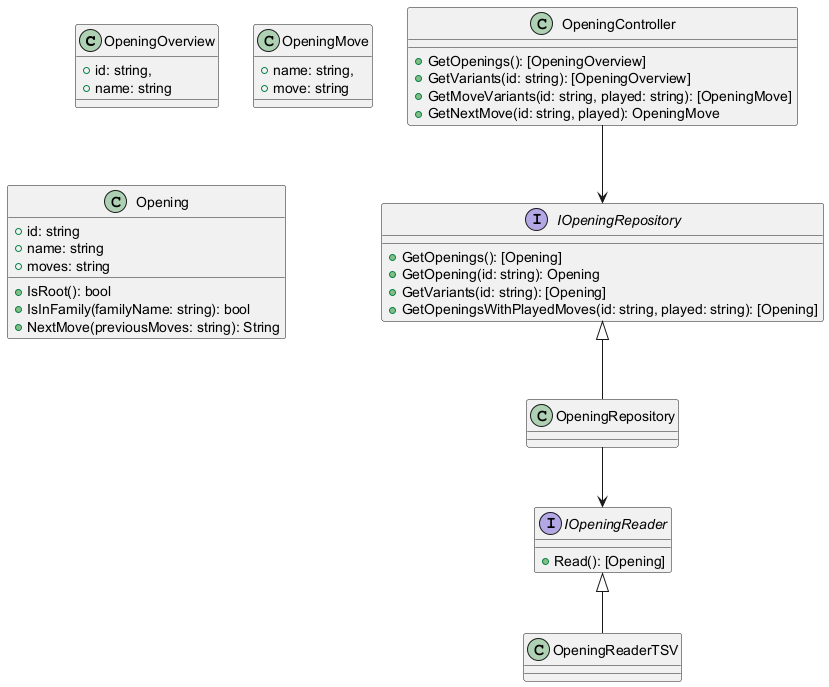
\includegraphics[width=\linewidth]{images/diagrams/opening.png}
  \caption{Klassendiagramm Eröffnungen}
  \label{fig:cd_opening}
\end{figure}

\begin{itemize}
  \item \lstinline|GET /openings| $\rightarrow$ GetOpenings
  \item \lstinline|GET /openings/{id}/variant| $\rightarrow$ GetVariants
  \item \lstinline|GET /openings/{id}/variant/next-moves| $\rightarrow$ GetMoveVariants
  \item \lstinline|GET /openings/{id}/next-move| $\rightarrow$ GetNextMove
\end{itemize}

Der Endpunkt \lstinline{GET /openings} liefert eine Liste mit allen Wurzeleröffnungen in Form von OpeningOverview-Objekten, die jeweils den Namen und die ID einer Eröffnung enthalten.
Eine Eröffnung wird in dem verwendeten Datensatz dann als Wurzeleröffnung kategorisiert, wenn der Name keinen Doppelpunkt enthält.

Der Endpunkt \lstinline|GET /openings/{id}/variant| ist dazu da alle Eröffnungen einer Eröffnungsfamilie zu bekommen. Eine Eröffnung gilt als zugehörig zu dieser Familie, wenn sie mit dem selben Namen beginnt, wie die im Pfad angegebene Eröffnung. Zum Beispiel besitzt die Eröffnung mit der ID D20 den Namen \enquote{Queen's Gambit Accepted}. Das bedeutet alle Eröffnungen, die mit \enquote{Queen's Gambit Accepted} beginnen gehören zu dieser Familie.

Der Endpunkt \lstinline|GET /openings/{id}/next-move| gibt ein OpeningMove-Objekt zurück, dass den Namen der Eröffnung und den nächsten Zug enthält. Bei diesem Endpunkt kann zusätzlich das Query-Parameter played übergeben werden mit den bisher gespielten Zügen im \ac{UCI}-Format. Wenn alle Züge gespielt wurden, wird ein leerer String als Zug übergeben.

Der Endpunkt \lstinline|GET /openings/{id}/variant/next-moves| dient dazu alle möglichen nächsten Züge in einer Eröffnungsfamilie herauszufinden. Er gibt alle OpeningMove-Objekte der gegebenen Eröffnungsfamilie zurück. Auch hier kann man das Query-Parameter played mitgeben. Die Liste enthält dann nur noch die Eröffnungen, die auch mit den angegebenen Zügen beginnen. Beispielsweise werden bei der Anfrage \lstinline|GET /openings/D20/variant?played=d2d4| nur Eröffnungen zurückgegeben, die mit dem Name \enquote{Queen's Gambit Accepted} beginnen und mit dem Zug \lstinline|d2d4| starten.

% Die Zuordnung zu einer Eröffnungsfamilie findet statt, wie in \autoref{cp:opening list} beschrieben.

\subsubsection{OpeningRepository}
Opening ist die Model Klasse. Sei enthält alle benötigten Daten zu einer Eröffnung. Die API gibt bei einer Anfrage entweder Instanzen der Klassen OpeningOverview oder OpeningMove zurück, die einen Teil der Informationen von Opening besitzen. Dadurch wird Bandbreite gespart und der Client bekommt nur die Daten, die er auch benötigt. Der Datenspeicher ist eine TSV-Datei, die von dem Lichess Datensatz abgeleitet wurde. Die ID wurde erstellt aus dem ECO-Code ergänzt durch einen Hash des englischen Namens. Bei identischer ID wurde immer die erste Variante ausgewählt.
Der Datensatz wird über das Repository Pattern abgefragt. IOpeningRepository enthält also alle Funtionen, um die Daten abzufragen und zu strukturieren, wie sie der OpeningController benötigt. Die OpeningRepository verwendet wiederum den IOpeningReader, welcher das Lesen der TSV-Datei abstrahiert. Auf diese Weise kann die TSV-Datei ohne viel Aufwand durch eine CSV- oder JSON-Datei ausgetauscht werden. Dafür muss lediglich eine entsprechende Implementierung für den IOpeningReader erstellt werden.

\subsection{SQL-Datenbank}
Die dynamischen Daten werden in einer relationalen SQL-Datenbank gespeichert. Dazu zählen die Logindaten der Nutzer und die Nutzerstatistiken zu den Eröffnungen. Dafür existieren die zwei Tabellen User und TrainingResult, welche nachfolgend in Relationenschreibweise notiert sind, wobei der Primärschlüssel fett gedruckt ist und der Fremdschlüssel kursiv:

\begin{itemize}
  \item User(\textbf{Id}, Name, PasswordHash)
  \item TrainingResult(\textbf{Id}, \textit{UserId}, OpeningId, Errors, Hints, DateTime)
\end{itemize}

Die Usertabelle existiert um das Einloggen und Registrieren zu ermöglichen. Mit einem Benutzernamen und einem Passwort kann sich ein Nutzer anmelden. Der Name besitzt aus diesem Grund einen Unique Constriant. Das Passwort wird in gehashter Form gespeichert. Für die Statistiken werden die Ergebnisse der Trainings gespeichert. Es wird gespeichert, wer das Training ausgeführt hat, für welche Eröffnung das Training ist, wie viele Fehler gemacht wurden, wie viele Hinweise benötigt wurden und zu welchem Zeitpunkt das Training ausgeführt wurde. OpeningId ist in diesem Fall kein Fremdschlüssel, da die Eröffnungen nicht in der relationalen Datenbank abgespeichert sind, sondern in einer separaten TSV-Datei. Mithilfe dieser Daten können durch SQL-Abfragen weitere Statistiken erstellt werden.

Für den Datenbankzugriff wird ein \ac{ORM} verwendet. Microsoft bietet in C\# dafür das Entity Framework Core an. Der Vorteil eines \ac{ORM}s ist, dass es den Zugriff auf die Datenbank abstrahiert. Zwischen verschiedenen SQL-Datenbanken gibt es einige Unterschiede, auf die geachtet werden muss, beim Schreiben von reinem SQL. Ein \ac{ORM} abstrahiert diese Unterschiede, indem der Zugriff und die Tabellenstruktur in der Sprache des ORM-Frameworks beschrieben wird, in diesem Fall C\#. Ein weiterer Vorteil ist, dass \ac{ORM}s vor einigen Fehlern, wie zum Beispiel Query-Injection schützen. Das Entity Framework Core besitzt zudem ein robustes System für Datenbankmigrationen. So ist es möglich Tabellenstrukturen auch im Nachhinein zu ändern und die Datenbanken mit geringem Risiko zu migrieren. Mit dem Entity Framework Core kann man zwischen vielen SQL-Datenbanken wählen. Für dieses Projekt wird PostgreSQL verwendet, da sie weit verbreitet ist und bekannt für ihre Stabilität.

\subsection{Authentifizierung}
Wie bereits in \autoref{cp:auth} beschrieben, wird auch in diesem Projekt eine Authentifizierung der Nutzer benötigt, um nutzerbezogene Statistiken zu sammeln und eine personalisierte Erfahrung zu bieten, und um den Zugriff auf die Schachengine zu begrenzen. \autoref{fig:cd_auth} beschreibt die Klassen, die bei der Authentifizierung verwendet werden. Der \lstinline{UserController} implementiert die folgende Endpunkte:

\begin{figure}[htb]
    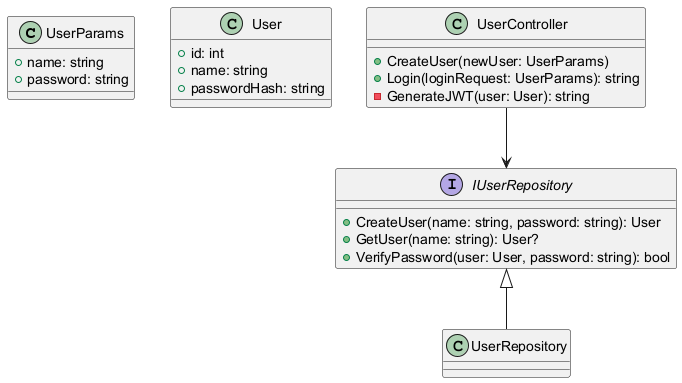
\includegraphics[width=\linewidth]{images/diagrams/auth.png}
    \caption{Klassendiagramm Authentifizierung}
    \label{fig:cd_auth}
\end{figure}

\begin{itemize}
    \item \lstinline{POST /users} $\rightarrow$ CreateUser
    \item \lstinline{POST /users/login} $\rightarrow$ Login
\end{itemize}

Über den ersten Endpunkt geschieht die Registrierung. Das Frontend schickt mit einer POST Anfrage UserParams mit dem Nutzername und Passwort das verwendet werden soll. Durch den Unique Index auf dem Nutzernamen ist es später möglich sich mit Name und Passwort zu authentifizieren.
Wenn der angegebene Nutzername bereits existiert, wird eine Fehlermeldung mit dem Code 409 (Conflict) geschickt, da es sich um einen semantischen Fehler handelt und die Anfrage im Konflikt mit dem Zustand des Servers steht. %todo richtigen Fehlercode im Code verwenden
Wenn der Nutzer noch nicht existiert, wird er mithilfe der Klasse UserRepository angelegt.
% Sie verwendet den Passworthasher von ASP.NET Core, welcher eine sichere Hashfunktion mit Salt verwendet, um die Passwörter sicher zu speichern.
Zur sicheren Speicherung der Passwörter wird der Passwort-Hasher von ASP.NET Core verwendet, der eine sichere Hashfunktion mit einem zufällig generierten Salt verwendet.

Die erste Authentifizierung wird über den Controller-Endpunkt \lstinline{POST /users/login} durchgeführt. Dafür muss der eindeutige Nutzername und das Passwort angegeben werden. Der UserController kann mithilfe des UserRepositorys überprüfen, ob der Nutzer existiert und ob das angegebene Passwort richtig ist. Falls der Nutzer nicht existiert wird der Fehlercode NotFound (404) zurückgegeben und falls das Passwort nicht stimmt wird Unauthorized (401) zurückgegeben.
Andernfalls wird über die Funktion GenerateJWT ein \ac{JWT} erstellt. Dieses Token enthält die User ID und den Ablaufzeitpunkt, welcher initial zwei Stunden in der Zukunft liegt. Der Ablaufzeitpunkt ist wichtig, damit das Token nicht auf unbestimmte Zeit gültig bleibt und somit ein Sicherheitsrisiko birgt. Weitere Informationen und komplexere Nutzerrollen sind in dieser Anwendung nicht notwendig. Mithilfe von diesem Token kann der Nutzer die weiteren Endpunkte verwenden, die auch eine Authentifizierung benötigen. Das ist bei allen der Fall, außer bei den Endpunkten des UserControllers, um die Angriffsfläche zu minimieren.

\subsection{Statistiken}
Um die Benutzererfahrung zu personalisieren werden Statistiken in Form von Trainingsergebnissen gesammelt. Die Trainingsergebnisse können verwendet werden, um verschiedene Kennwerte zu berechnen, zum Beispiel, wie viele Fehler der Nutzer im Durchschnitt bei einer Eröffnung macht. Die Kennwerte können dem Nutzer angezeigt werden, damit dieser einschätzen kann, wie gut er eine Eröffnung beherrscht. Zusätzlich dazu werden die Kennwerte verwendet, um einen Wert zu berechnen, der angeben soll, wie gut der Spieler eine Eröffnung kann. Dieser Wert wird Expertise genannt und gibt an, mit welcher Wahrscheinlichkeit ein Nutzer die Eröffnung fehlerfrei nachspielt. Um diese Funktionalitäten bereitzustellen, werden die Klassen aus \autoref{fig:cd_stats} implementiert.

\begin{figure}[h]
    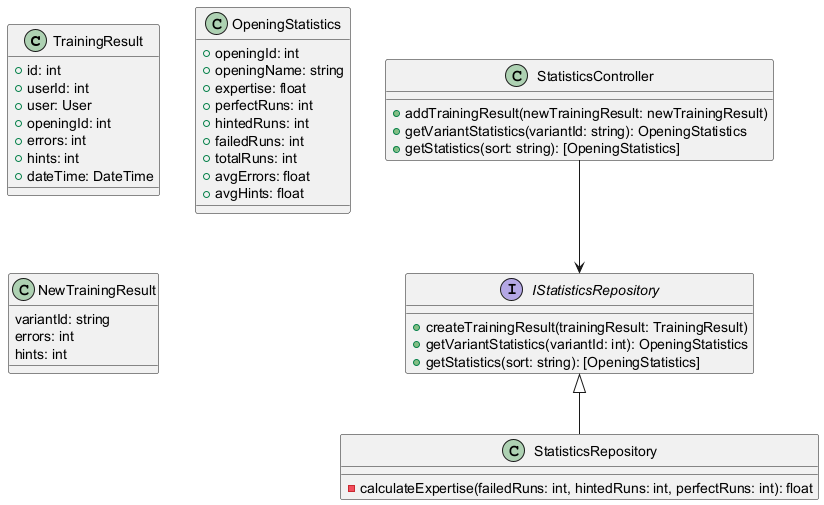
\includegraphics[width=\linewidth]{images/diagrams/stats.png}
    \caption{Klassendiagramm Statistiken}
    \label{fig:cd_stats}
\end{figure}


\subsubsection{StatisticsController}
Der StatisticsController übernimmt die Bereitstellung folgender Endpunkte:

\begin{itemize}
  \item \lstinline|POST /stats/variants| $\rightarrow$ AddTrainingResult
  \item \lstinline|GET /stats/variants/{id}| $\rightarrow$ GetVariantStatistics
  \item \lstinline|GET /stats/variants| $\rightarrow$ GetMoveVariants
\end{itemize}

Während dem Übungsmodus zählt das Frontend mit, wie viele Fehler der Spieler macht und wie viele Tipps er verwendet. Sobald der Nutzer das Training beendet, werden diese Daten über den Endpunkt \lstinline{POST /stats/variants} an das Backend geschickt. Das erkennt durch das \ac{JWT} den Nutzer und ergänzt die Daten durch die UserID und den aktuellen Zeitstempel, bevor sie über das IStatisticsRepository in die Tabelle TrainingResult geschrieben werden.

Eine Ausgabe der TrainingResults gibt es nicht, da es alleinstehend nicht sonderlich interessant ist. Stattdessen können berechnete Statistiken abgefragt werden. Über \lstinline|GET /stats/variants/{id}| werden die Statistiken einer einzelnen Eröffnungsvariante abgerufen und über \lstinline|GET /stats/variants| bekommt man eine Liste aller bisher geübten Eröffnungen mit ihren Statistiken. Um Nutzern eine Empfehlung zu geben, welche Eröffnungen als nächstes geübt werden sollen, kann man die Eröffnungen nach der Expertise sortieren. Je höher eine Eröffnung in dieser Liste ist, umso mehr sollte sie wieder geübt werden. Die Berechnungen für die Expertise werden im StatisticsRepository durchgeführt.

\subsubsection{StatisticsRepository}
Die Klasse OpeningStatistics enthält alle statistischen Werte, die das StatisticsRepository berechnet.
% An der Klasse OpeningStatistics kann man erkennen, welche Statistiken berechnet werden.
% Welche Werte berechnet werden kann in der Klasse OpeningStatistics gesehen werden.
Besonders interessant ist hier der Wert \enquote{expertise}, welcher angeben soll, mit welcher Wahrscheinlichkeit ein Nutzer die Eröffnung fehlerfrei wiedergeben kann.
Die Berechnung dieses Wertes basiert auf der Halbwertszeitregression aus \autoref{cp:halbwertszeitregression}.

% Die TrainingResults können verwendet werden, um einzuschlätzen, wie gut der Nutzer eine Eröffnung kann. Aufgrund dessen ist es möglich, dem Nutzer eine Empfehlung zu geben, welche Eröffnung er als nächstes üben soll. Man kann dafür Halbwertszeitregression aus \autoref{cp:halbwertszeitregression} anwenden.
% Dieser Algorithmus ist allerdings aufwendig zu implementieren und es werden Datensätze benötigt, die beschreiben, wie schnell Schacheröffnungen gelernt und vergessen werden. Aus diesem Grund wird diese Lösung im Rahmen dieser Arbeit nicht implementiert.

Wie bei der Halbwertszeitregression ist die Vergessenskurve $p = 2^{-\Delta/h}$ die Basis, wobei $p$ als der Expertisenwert zu verstehen ist. Für $\Delta$ kann die Dauer eingesetzt werden, seitdem das letzte Training durchgeführt wurde.
Die Halbwertszeit $h$ wird auch durch die Funktion $\hat{h}_\Theta = 2^{\Theta*x}$ bestimmt.
Die Bestandteile des Merkmalsvektors $x$ und seinen Gewichtungen $\Theta$ sind in \autoref{tab:featurevector} zu sehen.
In den TrainingResults werden noch weitere Daten gesammelt, damit man später die Flexibilität hat, andere Merkmale zu verwenden, wie zum Beispiel die durchschnittlichen Fehler pro Trainingsdurchlauf.
Im Gegensatz zur Halbwertszeitregression wird keine Regression durchgeführt, um den Gewichtsvektor $\Theta$ zu bestimmen, weil das ein erheblicher Zusatzaufwand wäre und Datensätze benötigt werden, die beschreiben, wie schnell Schacheröffnungen gelernt und vergessen werden. Die Gewichte werden stattdessen im Vorhinein festgelegt. Der Nachteil davon ist, dass sie nicht getestet sind und unklar ist, wie gut sie zu der tatsächlichen Vergessenskurve passen. Eine Festlegung durch empirisch erfasste Werte oder durch Regression bestimmte Werte könnten den Algorithmus deutlich verbessern.

\begin{table}[htb]
    \centering
    \begin{tabular}{|c|c|l|}
        \hline
        $\theta$ & $x$ & Beschreibung \\
        \hline
        -0,5 & $x_f$ & Anzahl der Trainingsdurchläufe mit Fehlern \\
        \hline
        0,2 & $x_t$ & Anzahl der fehlerfreien Trainingsdurchläufen mit Tipps \\
        \hline
        0,6 & $x_p$ & Anzahl der perfekten Trainingsdurchläufe ohne Tipps und Fehler \\
        \hline
        0,1 & $x_n$ & Anzahl der gesamten Trainingsdurchläufe \\
        \hline
    \end{tabular}
    \caption{Merkmalsvektor und Gewichte}
    \label{tab:featurevector}
\end{table}

Mit den aktuellen Werten muss $\Delta$ in Tagen angegeben werden. In \autoref{fig:vergessenskurven} sind Vergessenskurven mit den angegebenen Gewichten und Beispielvektoren $x$ zu sehen. Bei vier fehlgeschlagenen und vier perfekten Trainingsdurchläufen fällt die Kurve in den ersten zehn Tagen stark ab und ist nach 8 Tagen bereits unter 10\%, wie in der unteren Kurve zu sehen. Nach einigen weiteren perfekten Durchläufen fällt die Kurve flacher ab. So ist nach diesem Modell 12 Tage später die Wahrscheinlichkeit noch über 80\%, dass der Nutzer die Eröffnung wieder fehlerfrei durchführt, was bei zehn perfekten Trainingsdurchläufen durchaus plausibel ist.

\begin{figure}[htb]
    
\begin{center}
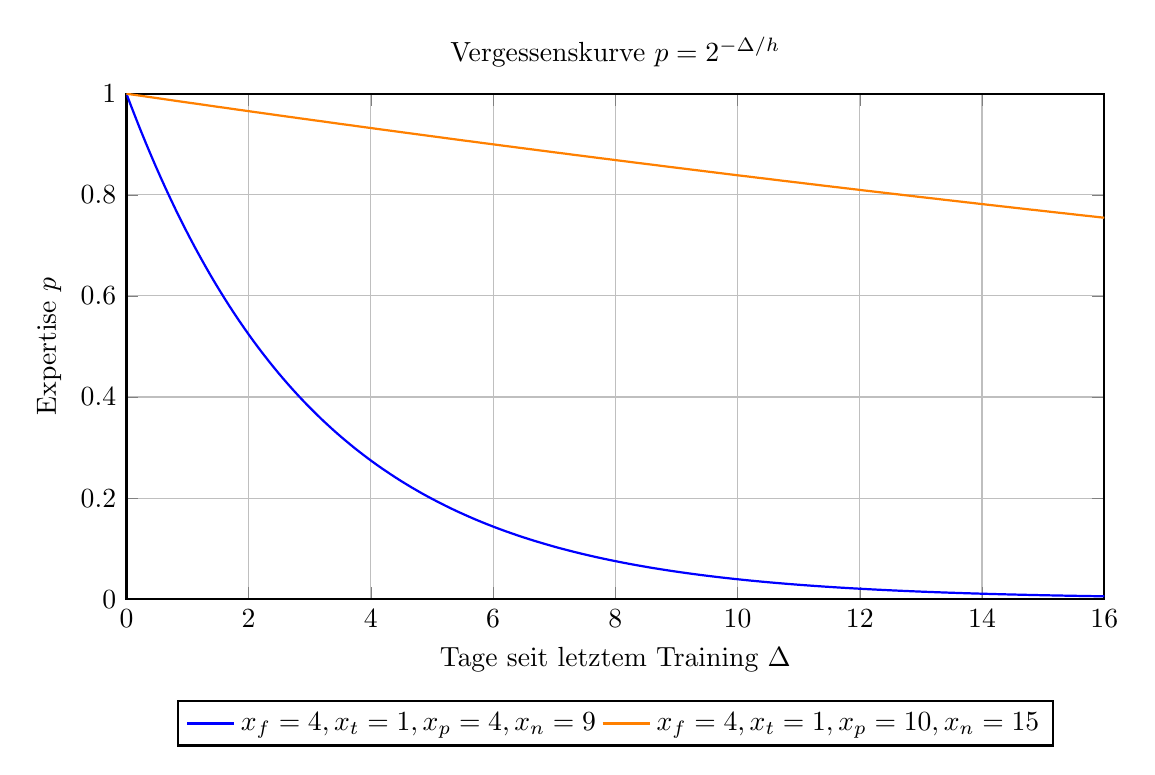
\begin{tikzpicture}
\begin{axis}[
    width=14cm,
    height=8cm,
    xlabel={Tage seit letztem Training $\Delta$},
    ylabel={Expertise $p$},
    xmin=0, xmax=16,
    ymin=0, ymax=1,
    samples=200,
    grid=major,
    thick,
    domain=0:16,
    legend style={at={(0.5,-0.2)}, anchor=north, legend columns=-1},
    title={Vergessenskurve $p = 2^{-\Delta / h}$}
]

% Parameter
\def\xf{4}
\def\xt{1}
\def\xp{4}
\def\xn{\xf+\xt+\xp}
\def\thetaf{-0.6}
\def\thetat{0.2}
\def\thetap{0.6}
\def\thetan{0.1}

% Berechnung der Halbwertszeit
\pgfmathsetmacro{\h}{
  2^((\thetaf)*(\xf) + (\thetat)*(\xt) + (\thetap)*(\xp) + (\thetan)*(\xn))
}
\pgfmathsetmacro{\g}{
  2^((\thetaf)*(\xf) + (\thetat)*(\xt) + (\thetap)*(10) + (\thetan)*(15))
}

% Plot der Vergessenskurve
\addplot[
    blue,
    thick
]
{2^(-x / \h)};
\addlegendentry{$x_f=\pgfmathprintnumber{\xf}, x_t=\pgfmathprintnumber{\xt}, x_p=\pgfmathprintnumber{\xp}, x_n=9$}

\addplot[
    orange,
    thick
]
{2^(-x / \g)};
\addlegendentry{$x_f=\pgfmathprintnumber{\xf}, x_t=\pgfmathprintnumber{\xt}, x_p=10, x_n=15$}

%\addlegendentry{$h = \pgfmathprintnumber[fixed, precision=2]{\h}$}

\end{axis}
\end{tikzpicture}
\end{center}

    \caption{Beispielhafte Vergessenskurve}
    \label{fig:vergessenskurven}
\end{figure}

\subsection{Schachengine}
Eine Schachengine mit \ac{UCI}-Protokoll kann eingebunden werden, indem ein Adapter geschrieben wird, der \ac{REST}-Anfragen für die Engine übersetzt. Das wird dadruch ermöglicht, dass REST und UCI keinen Zustand besitzen. Über einen Endpunkt, wie zum Beispiel \lstinline|GET /engine| könnte ein Computerzug angefragt werden. Über Query-Parameter played und level müsste das Frontend die bisher gespielten Züge übertragen und die Stärke der Engine. Aus Zeitgründen wurde im finalen Programm keine Schachengine eingebunden.

\section{Laufzeitsicht}

In diesem Kapitel wird der Ablauf von den komplexeren Funktionen der Anwendung beschrieben. Dabei wird erklärt, welche Anfragen das Frontend schickt und wie die REST-Endpunkte dabei verwendet werden.

\subsection{Lernmodus}
Für den Lernmodus werden die Funktionen unter dem Endpunkt \lstinline{/openings} aus \autoref{cp:openings} verwendet.
Das Sequenzdiagramm in \autoref{fig:sd_opening_training} zeigt den Ablauf des Lernmodus. Er kann in den folgenden drei Schritten beschrieben werden.

\begin{enumerate}
     \item Als erstes wählt der Nutzer den Lernmodus aus. Das Frontend schickt dann eine GET Anfrage an den Endpunkt \lstinline{/openings}. Dieser liefert eine Liste von OpeningOverviews, die die Namen und IDs der Wurzeleröffnungen enthalten. Die Namen werden dem Nutzer zur Auswahl gezeigt.
     \item Angenommen der Nutzer wählt die Eröffnung mit der ID D20 aus, dann schickt das Frontend eine GET Anfragen an den Endpunkt \lstinline|/openings/D20/variants/next-moves|. Daraufhin liefert die API ein OpeningMove-Objekt für jede Eröffnung, die mit dem selben Namen anfangen, wie die Eröffnung mit der ID D20. Die OpeningMove-Objekte enthalten den Namen und den ersten Zug der jeweiligen Eröffnung. Diese werden dem Nutzer angezeigt.
     \item Der Nutzer kann anschließend auswählen, welchen Zug er ausführen möchte, zum Beispiel 1. d4. Die darauffolgenden Züge können wiederum mit der folgenden GET Anfrage herausgefunden werden: \lstinline|/openings/D20/variants/next-moves?played=d2d4|. Hier werden die bereits ausgeführten Züge im Query-Parameter \lstinline{played} mit \ac{UCI}-Format übergeben. Die API liefert dann nur noch die Eröffnungen, die auch mit den selben Zügen beginnen. Dieser Schritt wird so oft wiederholt, bis keine weiteren Züge mehr vorhanden sind, also die Liste mit OpeningMoves leer ist.
\end{enumerate}

\begin{figure}[p]
    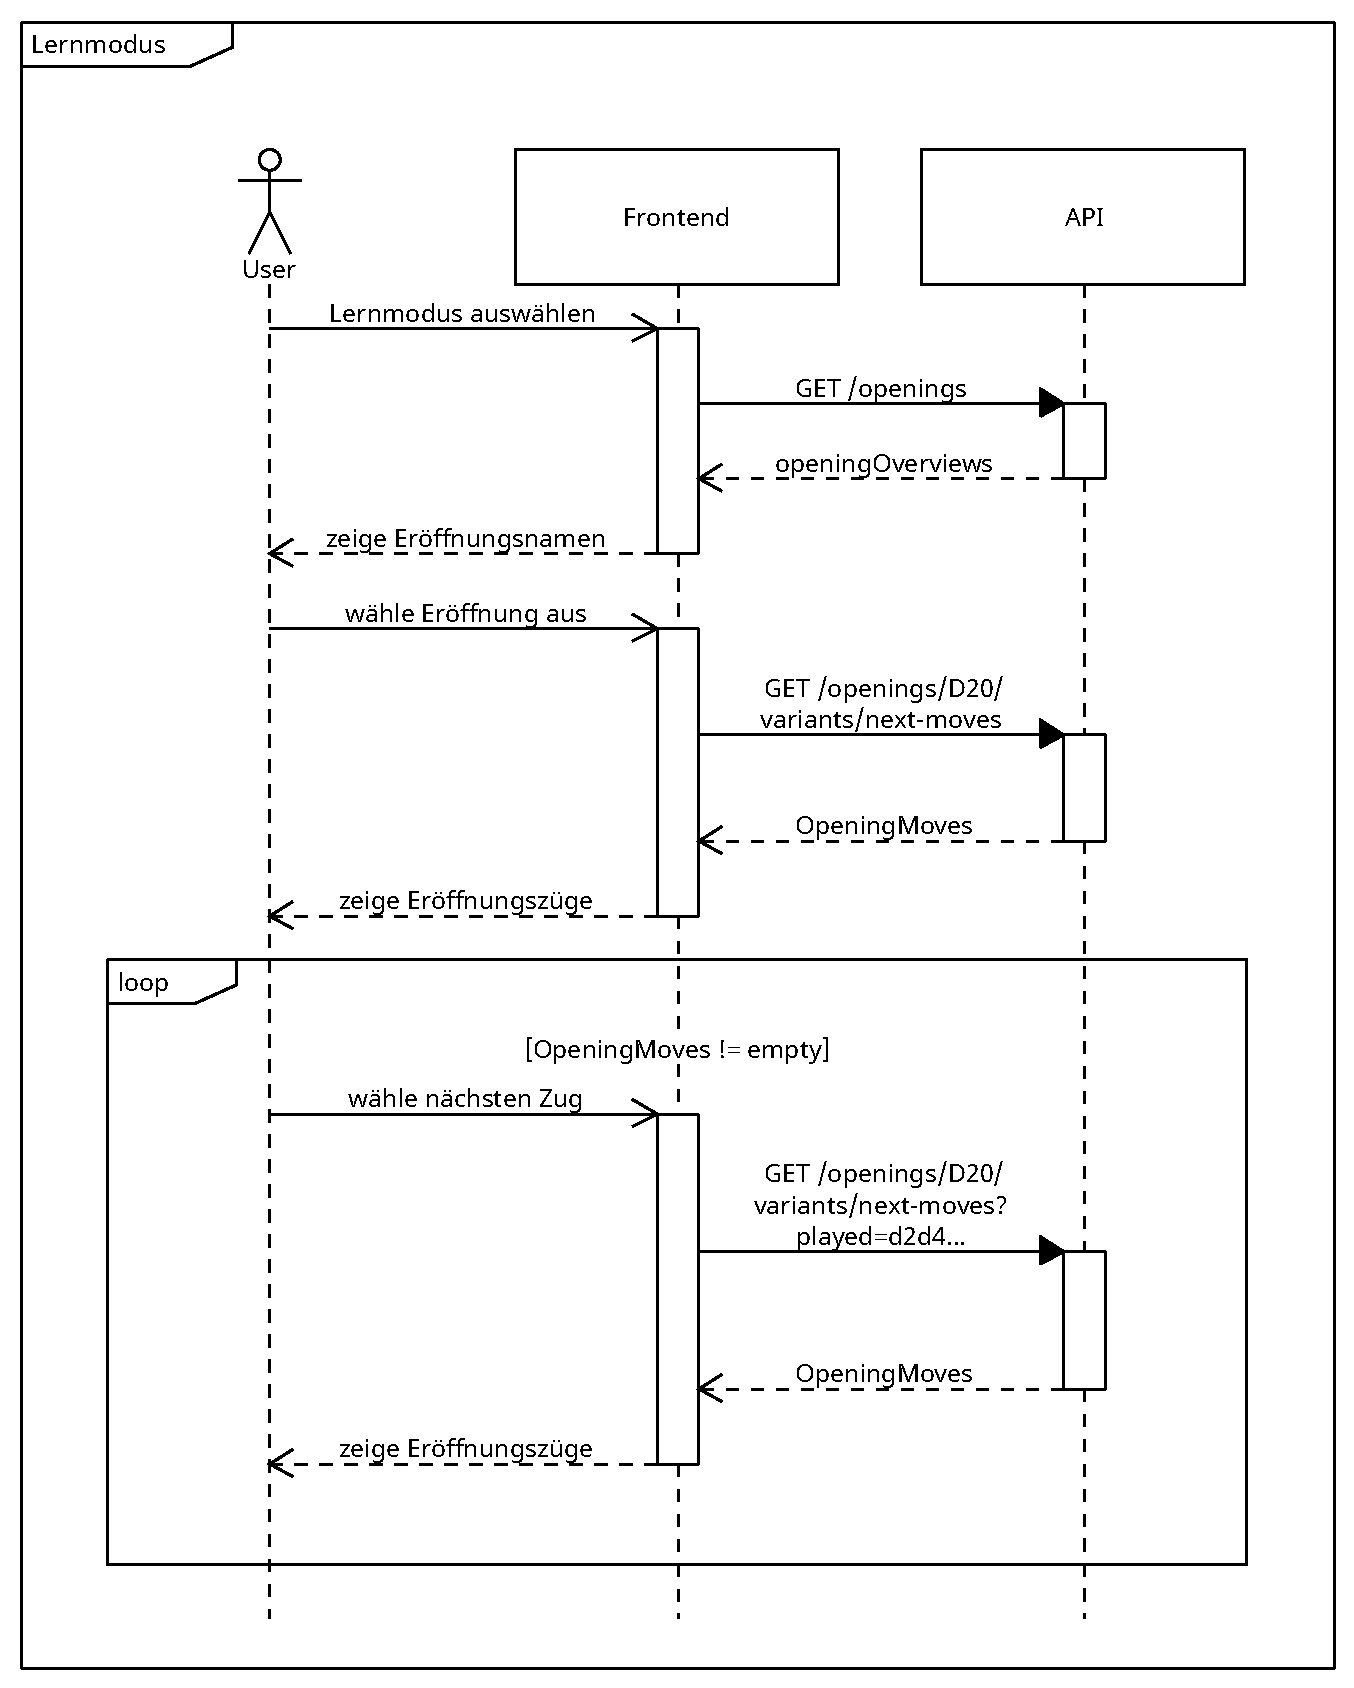
\includegraphics[width=\linewidth]{images/diagrams/sd_opening_training}
    \caption{Ablauf Übungsmodus}
    \label{fig:sd_opening_training}
\end{figure}

\clearpage

\subsection{Übungsmodus}
Der Übungsmodus verwendet ähnliche Endpunkte, wie der Lernmodus. Statt dem Endpunkt \lstinline|/openings/{id}/variants/next-moves| wird hier der Endpunkt \lstinline|/openings/{id}/next-move| verwendet, da die unterschiedlichen Varianten nicht betrachtet werden müssen. Der Ablauf wird in dem Zustandsdiagramm in \autoref{fig:sd_training} dargestellt, da dieser Ablauf etwas komplexer ist. Es ist jedoch zu erwähnen, dass der Zustand sich ausschließlich im Frontend befindet, um der REST Architektur treu zu bleiben. Alle benötigten Zustandsinformationen werden mit jeder Anfrage an das Backend mitgegeben.

\begin{enumerate}
    \item \textbf{Eröffnungswahl:} Als erstes wählt der Nutzer den Übungsmodus aus und das Frontend holt sich wieder über \lstinline{GET /openings} die Liste der Wurzeleröffnungen und zeigt diese mit Namen an.
    \item \textbf{Variantenwahl:} Nachdem der Nutzer eine ausgewählt hat, muss er eine der Varianten auswählen, die über \lstinline|GET  /openings/{id}/variants| zurückgegeben werden und entscheiden ob er die schwarzen Figuren oder die weißen spielen will. Bei Auswahl der weißen Figuren geht es mit dem Spielerzug weiter, bei Auswahl der schwarzen mit dem Computerzug.
    \item \textbf{Spielerzug:} Für den nächsten Zug wird der Nutzer aufgefordert, ihn auszuführen. Das Frontend fragt daraufhin mit dem Endpunkt \lstinline|GET /openings/{id}/next-move| ab, was der richtige nächste Zug für diese Eröffnung ist. Wenn die Züge nicht übereinstimmen, wird er aufgefordert es erneut zu versuchen. An dieser Stelle kann auch die Hinweisfunktion implementiert werden. Wenn der Nutzer nach einem Hinweis fragt, kann das Frontend über den selben Endpunkt den richtigen Zug abfragen und einen Hinweis geben, zum Beispiel welche Figur bewegt werden muss. Dafür ist kein zusätzlicher Endpunkt in der API notwendig. Wenn der Nutzer den richtigen Zug gefunden hat und es noch weitere Züge gibt, geht es mit dem Computerzug weiter. Falls es keine weiteren Züge mehr gibt folgt der Schritt Training speichern.
    \item \textbf{Computerzug:} Der nächste Zug wird vom Computer ausgeführt. Dafür holt sich das Frontend den Zug über den Endpunkt \lstinline|GET /openings/{id}/next-move| und führt ihn aus. Wenn das der letzte Zug war geht es mit dem Training speichern weiter, ansonsten ist der Nutzer wieder an der Reihe und es geht mit dem Spielerzug weiter.
    \item \textbf{Training speichern:} Nach dem letzten Zug wird ein TrainingResult angelegt mit der Anzahl an Fehlern und Hinweisen, über den Endpunkt \lstinline|POST /stats/variants|.
\end{enumerate}

\begin{figure}[h]
    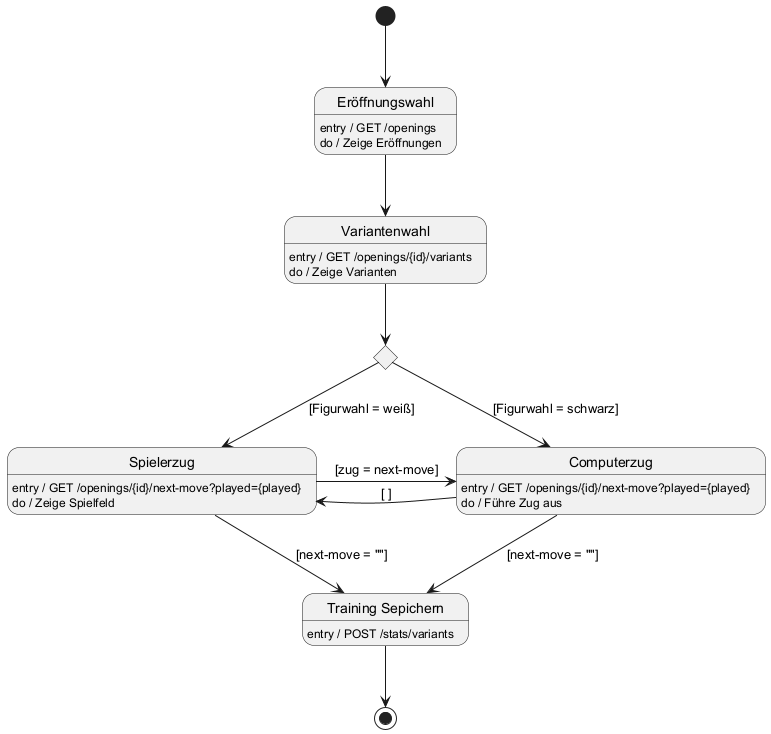
\includegraphics[width=\linewidth]{images/diagrams/sd_training}
    \caption{Ablauf Trainingsmodus}
    \label{fig:sd_training}
\end{figure}

\clearpage

\section{Verteilungssicht (Deployment)}
Um das Programm auf einem Server bereitzustellen werden die einzelnen Bestandteile in Docker Images eingebettet. Das hat vor allem den Vorteil, dass die Programme auf allen Plattformen, die Docker unterstützen, unkompliziert ausgeführt werden können. Die einzelnen Images können mittels Docker-Compose gestarten und verbunden werden. Diese Anwendung ist in drei Images aufgeteilt, die auch in \autoref{fig:deployment} zu sehen sind. Ein Image enthält das Frontend, eins die Rest-API und eins die Postgres Datenbank. Die Datei mit den Eröffnungen wird in das Image der Rest-API integriert und ist daher nicht auf dem Diagramm zu sehen. Das Frontend und die API ist durch einen Reverse Proxy über das Internet erreichbar. Das ermöglicht es, dass die Komponenten auch auf unterschiedlichen Servern ausgeführt werden können.
 
\begin{figure}[h]
    \centering
    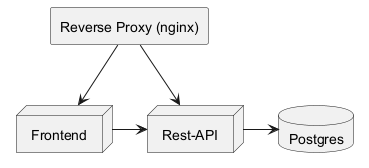
\includegraphics[width=10cm]{images/diagrams/deployment}
    \caption{Verteilungssicht}
    \label{fig:deployment}
\end{figure}

